\chapter{Radio Astronomy and the Rotation of the Galaxy (Small Radio Telescope)}

%TODO Add information on how students can infer existance of dark matter from rotation curve

\section{Assessment}

Your lab report will be assessed based on answering lab questions correctly and with justification (showing work or giving reasoning) and the following rubric rows found in Appendix~\ref{cha:rubrics}: A11, F2, G4, G5.

\section{Changes to the lab write-up}

The lab write-up is included below, and the following changes should be made to it.

\subsection{Operating the small radio telescope (page 3)}

The telescope is mounted 3\textdegree{} azimuth out of alignment. Each time the SRT program is loaded, the following command must be run to compensate for this, before any useful observations can be made.

\begin{itemize}
	\item Click on the ``\texttt{offset}'' button in the top row.
	
	\item Type ``\texttt{3.0 0.0}'' and press enter.
\end{itemize}

\subsection{Calibration in practice (page 5)}

For calibration, set the frequency to 1424 MHz, not 1416 MHz. Therefore, for the first \textbf{Lab Task}, you will type ``\texttt{1424 1}'' instead of ``\texttt{1416 1}''.

\subsection{Background Noise (page 6)}

\textbf{Lab tasks}: Again, the frequency should be 1424 MHz, not 1416 MHz.

\section{Lab write-up}

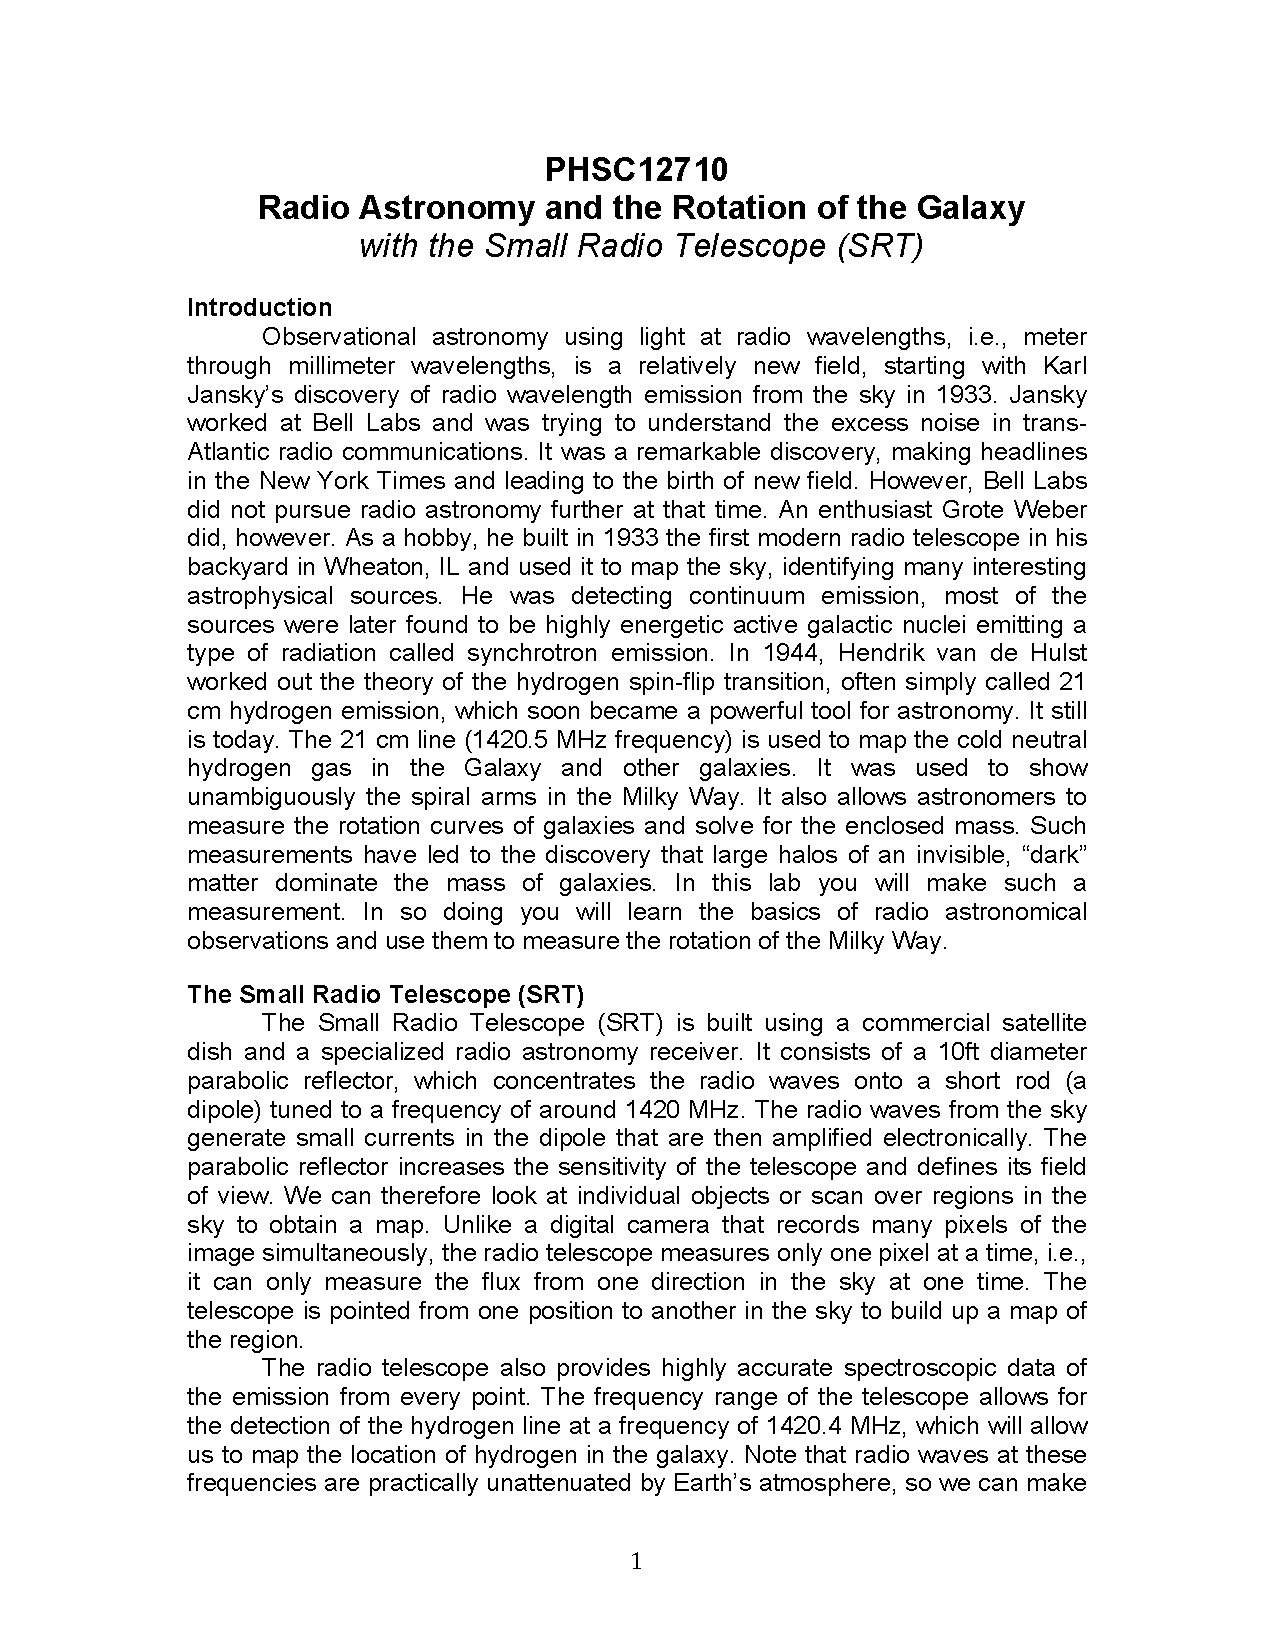
\includepdf[pages=-]{galaxy-rotation-srt/MilkyWayLab2018.pdf}